メソMD解析で得られた組織構造を定量的に特徴づけるために,次の4つの分布を求める.
\begin{itemize}
	\item X線回折(X-ray diffraction:XRD)パターン
	\item 動径分布関数(Radial distribution function:RDF)
	\item 局所密度分布
	\item 粗視化粒子方向の確率密度分布
\end{itemize}
以下では,これらの分布関数の定義と求め方を示す.
\subsection{X線回折(XRD)パターン}
試料で散乱されたX線の観測方向による強度変化のプロットはX線回折パターンと呼ばれる.
X線源がmonochromaticな平面波を照射していると仮定するとき,位置$\fat{x}$における
入射X線$u(\fat{x})$は,波数ベクトル$\fat{k}^{in}$を用いて
\begin{equation}
	u^{in}(\fat{x})=I_0 \exp(i\fat{k}^{in}\cdot\fat{x})
	\label{eqn:uin}
\end{equation}
と表すことができる.今,試料を構成する物質の作る電荷密度分布を$\gamma(\fat{x})$,
散乱X線の波数ベクトルを$\fat{k}_{sc}$とすれば,無限遠方で観測される散乱X線を
\begin{equation}
	u^{sc}(2\theta)=I_0 \int \gamma(\fat{x})\exp(i\fat{k}\cdot\fat{x})d\fat{x}, \ \ 
	\left(\fat{k}=\fat{k}^{sc}-\fat{k}^{in}\right)
	\label{eqn:usc}
\end{equation}
と表すことができる.
ただし$2\theta$は$\fat{k}^{in}$と$\fat{k}^{sc}$が成す角を表す.
X線計測で実際に測定することができるのはX線強度だけである.
散乱X線の強度は,式(\ref{eqn:usc})の絶対値をとり$\left| u^{sc}(2\theta)\right|$で,
与えられ,
\begin{equation}
	\left|u^{sc}(2\theta)\right|
	=
	I_0\left|\int \gamma(\fat{x}) \exp(i\fat{k}\cdot \fat{x}) d\fat{x} \right|
	\label{eqn:I2th_bar}
\end{equation}
と書くことができる.式(\ref{eqn:I2th_bar})の量は,入射X線の伝播方向$\varphi$にも依存するので,
\begin{equation}
	I_\varphi(2\theta):
		=\frac{\left|u(2\theta)\right|}{I_0}
		=
	\left|\int \gamma(\fat{x}) \exp(i\fat{k}\cdot \fat{x}) d\fat{x} \right|
	\label{eqn:Iphi}
\end{equation}
と表すことにする.
メソMD解析で得られる組織構造は,粘土試料のごく一部を表すものと言える.
従って,実際のX線回折試験で用いる粘土試料には,メソMDシミュレーションで得られたような
組織構造が,様々な方向を向いて含まれていると考える必要がある.このことは,試料からみて
X線はあらゆる方向から入射されると言い換えることができ,その時に観測される散乱X線の
強度$I(2\theta)$は,式(\ref{eqn:Iphi})を$\varphi$について積分した
\begin{equation}
	I(2\theta)=\int I_{\varphi}(2\theta) d\varphi
	\label{eqn:XRD}
\end{equation}
となる.従って,メソMDで得られた組織構造から電荷分布$\gamma(\fat{x})$を決定し,
式(\ref{eqn:Iphi})と式(\ref{eqn:XRD})の積分を評価すれば,シミュレーション結果に
対応したXRDパターンを合成することができる.
その際,式(\ref{eqn:Iphi})の積分は電荷密度分布$\gamma(\fat{x})$のフーリエ変換を
FFTで計算することによって得ることができる.本研究では,電荷密度$\gamma(\fat{x})$の
最も簡単なモデルとして,固相領域を表す次のような特性関数に平均電荷密度$\gamma_0$を乗じた
次のものを用いる
\begin{equation}
	\gamma(\fat{x})=\left\{
		\begin{array}{cc}
		\gamma_0 &  \fat{x} \in D_s \\
			0 &  otherwise
		\end{array}
	\right.
	\label{eqn:gamma}
\end{equation}
ただし,$D_s$は組織構造モデルにおいて粘土分子が占める固相領域を意味する.
このモデルでは,電荷が粘土分子内で均一に分布していると仮定されており,
粘土分子内での電荷の偏りに起因した散乱指向性や,水和水によるX線の
散乱の影響ともに無視されている.しかしながら,間隙水による散乱の影響は,
電荷量の割合からして,粘土分子による散乱よりも影響が小さいと考えられる.
また,粘土分子の内部構造に起因した散乱パターンは,観測方向$2\theta$が
比較的大きな範囲に現れるため,メソMD解析で興味の対象となる粘土分子の
積層構造に起因した回折ピークの位置や強度には影響が少ない.
以上のことからから,粘土分子の内部構造や間隙水分布を無視した電荷分布を用いても,
粘土の積層構造や膨潤状態を調べるためXRDパターンを合成する上で大きな支障はないと
考えられる.なお,メソMD結果からXRDパターンを合成する際には,$\gamma(\fat{x})$を
適当な空間解像度でピクセル画像として構成する.図\ref{fig:fig5}-(a)と(b)は
その一例を示したもので,(a)の図はメソMD解析で得られた組織構造を,
(b)はそれを,粘土分子の厚さを1nmとして固相領域$D_s$(黄色)と間隙領域$D_p$(紺)
に塗り分けたものである.このようにして作成した二値化画像$\gamma(\fat{x})$を,
空間変数についてフーリエ変換して波数スペクトル
\begin{equation}
	\Gamma(\fat{k})=\int \gamma(\fat{x}) e^{i\fat{k}\cdot\fat{x}} d\fat{x}
	\label{eqn:Gamma}
\end{equation}
を求めると,同図(c)のような結果が得られる.
波数スペクトル$\Gamma(\fat{k})$を,2次元の離散フーリエ変換で計算すれば,
全ての波数ベクトル$\fat{k}$に対して式(\ref{eqn:Iphi})右辺の値が得られる.
そこで,
図\ref{fig:fig5}-(c)のような$2\theta$に対して
波数ベクトル$\fat{k}=\fat{k}^{sc}-\fat{k}^{in}$を定め,
$\theta$を変化させて波数スペクトルをサンプリングおよび加算すれば,
式(\ref{eqn:Iphi})の$I_\varphi(2\theta)$が得られる.
波数空間におけるこのようなサンプリングと和の計算を入射方向$\varphi$を変えて行い,
その結果を重ね合わせることで,最終的にXRD試験で観測される回折パターン$I(2\theta)$
を合成することができる.
%--------------------
\begin{figure}[h]
	\begin{center}
	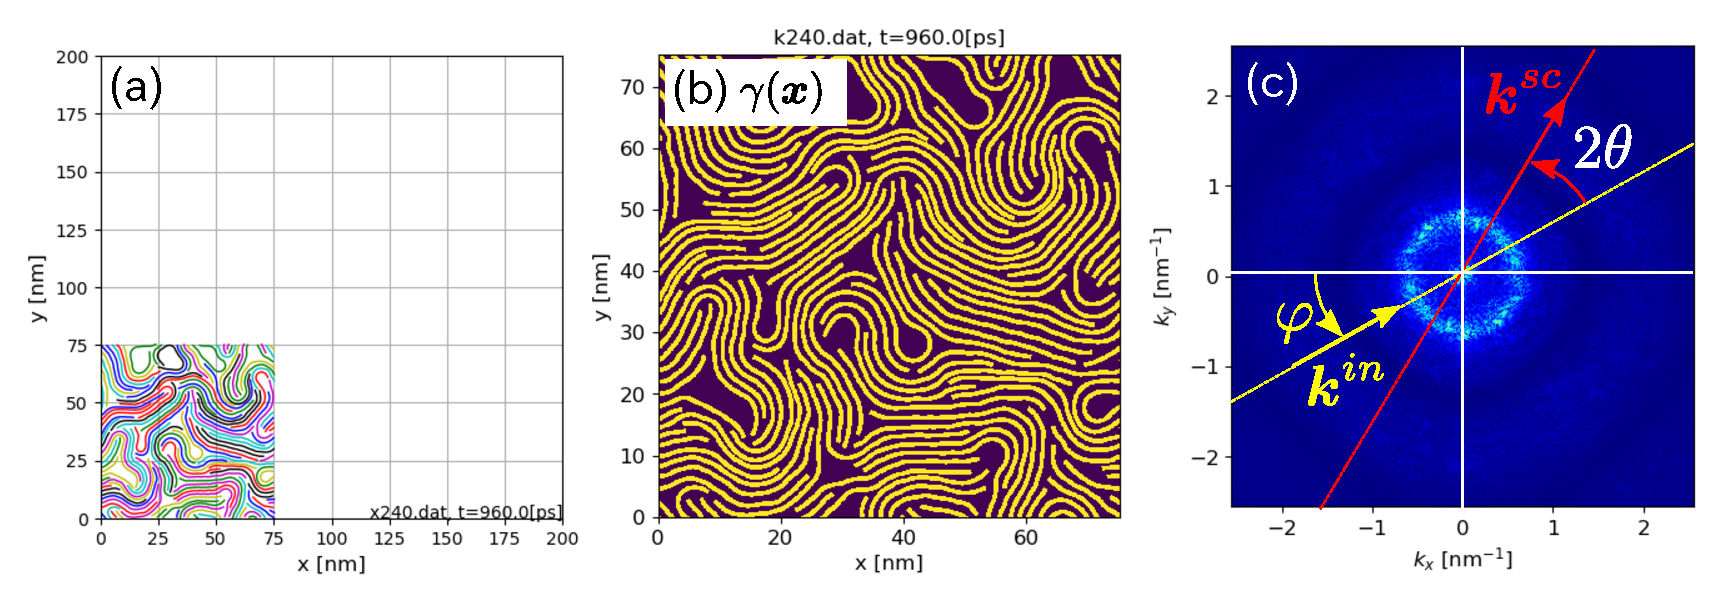
\includegraphics[width=1.0\linewidth]{Figs/fig5.eps} 
	\end{center}
	\caption{
		(a)メソMD計算で得られた組織構造モデル.
		(b)組織構造の二値化画像$\gamma(\fat{x})$. 
		(c)$\gamma(\fat{x})$の二次元フーリエ変換とX線の入射および散乱波数ベクトル.
	} 
	\label{fig:fig5}
\end{figure}
%--------------------
\subsection{動径分布関数}
動径分布関数(radial distribution function: RDF)は,着目粒子から一定距離離れた位置に
存在する粒子の数をカウントしたものである.より正確には,ある粒子を原点として測ったときの
動径距離$r$において,区間$[r,\Delta r)$に存在する粒子数を$g(r,r+\Delta r)$とするとき,
2次元空間における動径分布関数$f(r)$は
\begin{equation}
	f(r):=\frac{g(r,r+\Delta r)}{2\pi r}
	\label{eqn:RDF}
\end{equation}
で与えられる.ここで,第$i$番目の粗視化粒子の位置を$\fat{r}_i$とし,区間$[r,r+\Delta r)$で
1,そのほかの位置では0をとる矩形関数を
\begin{equation}
	U(r;\Delta r):=\left\{
		\begin{array}{cc}
			1 &  r \in [r;r+\Delta r)\\
			0 &  otherwise
		\end{array}
	\right.
	\label{eqn:}
\end{equation}
と表すと,$U(r;\Delta r)$を用いて$g(r,r+\Delta r)$次のように書くことができる.
\begin{equation}
	g(r,\,r+\Delta r)=\sum_{i\neq j} U(r_{ij}-r;\Delta r)
	\label{eqn:gr}
\end{equation}
ただし,
\begin{equation}
	r_{ij}=\left|\fat{r}_i-\fat{r}_j\right|
	\label{eqn:rij}
\end{equation}
とする.式(\ref{eqn:RDF})で定義されるRDFを組織構造解析にそのまま用いると,粘土分子を構成する
粗視化粒子の1次元的かつ規則的な配列に起因したピークが現れ,粘土分子の積層構造形成に関する情報
を読みとることができない.そこで,積層構造に寄与する粗視化分子が優先的にカウントされるよう,RDFの定義を以下のように修正する.

粗視化粒子$i$から粒子$j$を望む方向を指す単位ベクトルを
\begin{equation}
	\hat{\fat{r}}_{ij}=\frac{\fat{r}_j-\fat{r}_i}{r_{ij}}
	\label{eqn:rhat}
\end{equation}
と表す.各々の粗視化粒子は,それが属する粘土分子の情報を参照することで,
粒子の向きが定められる.粒子$i$の向きを,それが属する粘土分子全体の形状から
決定される法線ベクトル$\fat{n}_i$で定める.
このとき,
$\hat{\fat{r}}_{ij}\cdot\fat{n}_i$
と
$\hat{\fat{r}}_{ji}\cdot\fat{n}_j$
は,粒子$i$と$j$が近接していて同一分子に属するときには小さな値をとる傾向をもつ.
一方,2つの粒子が互いに積層した分子に属し,かつ近接している場合,これらは大きな
値を取る.そこで,粒子数をカウントする際に,これらの量で重み付けが行われるよう,
\begin{equation}
	f(r)=
	\sum_{i\neq j} \frac{U(r_{ij}-r;\, \Delta r)}{2\pi r}
	\left\{
		(\hat{\fat{r}}_{ij} \cdot \fat{n}_i)
		(\hat{\fat{r}}_{ji} \cdot \fat{n}_j)
	\right\}^2
	\label{eqn:RDFn}
\end{equation}
と動径分布関数を定義すれば,互いに積層する分子に属する粗視化粒子が,動径距離に
応じてどのように分布しているかを調べることができるRDFを構成することができる.
%%%%%%%%%%%%%%%%%%%
%%%%%%%%%%%%%%%%%
\subsection{数密度分布}
質点系を構成する第$i$番目の粒子の質量を$m_i$,位置を$\fat{r}_i$とすれば,
質量密度分布$\rho(\fat{x})$は,ディラクのデルタ関数を用いて
\begin{equation}
	\rho(\fat{x})=\sum_{i} m_i\delta\left(\fat{x}-\fat{r}_i\right)
\end{equation}
と表される.これを一般化した
\begin{equation}
	\rho(\fat{x})=\sum_{i} m_i w\left(\fat{x}-\fat{r}_i\right)
	\label{eqn:rhox_gen}
\end{equation}
を,組織構造解析のための局所密度として用いる.ただし,$w(\fat{x})$は
\begin{equation}
	\int w(\fat{x}) d\fat{x} =1
\end{equation}
と規格化された正またはゼロの重み関数を表す.
ここでは$w(\fat{x})$として,平均が0, 標準偏差が$\sigma$の2次元正規分布
\begin{equation}
	N(\fat{x};\sigma):=
	\frac{1}{2\pi\sigma^2}
	\exp\left(
		\frac{\left|\fat{x}\right|^2}{2\sigma^2}
	\right)
	\label{eqn:Gss2D}
\end{equation}
を用いる.これにより平滑化された密度場が得られ,さらに,式(\ref{eqn:Gss2D})
で$\sigma$を層間距離程度にとれば,積層した粘土分子層間は,層外の空隙よりも
高い密度をもつよう局所密度を与えることができる.
粘土分子層間と層外の間隙を区別することのできる,一般化された局所密度を定義する.
%粘土分子が占める領域を固相領域$D_s$,それ以外の間隙部を$D_p$とする.
%$D_s$における質量密度は粘土の密度$\rho_s$に一致し,$D_p$における密度は0とみなすことができる.
%すなわち,メソMD解析結果から与えられる局所密度$\rho(\fat{x})$は,特性関数$\gamma(\fat{x})$
%を用いて
%\begin{equation}
%	\rho(\fat{x})=\rho_s \gamma(\fat{x})
%\end{equation}
%と表すことができる.
\subsection{粘土分子方向の確率密度}
組織構造の配向は,拡散や透水等,物質輸送挙動の異方性に寄与すると予想される.
そこで,メソMD解析で得られた組織構造がもつ配向性を定量的に調べることを考える.
各粗視化粒子について,それが属する分子の情報を参照することで,粒子向きが定められることは
上に述べた通りである.そこで,粒子$i$の向きを単位ベクトル$\fat{n}_i$で表し,
その偏角を$\alpha_i = \alpha_i( \fat{n}_i)$と書く.
$\left\{ \alpha_i \right\}$のヒストグラムを求めて正規化すれば,
粒子方向$\alpha$の出現頻度を表す確率密度関数
\begin{equation}
	\Psi:=
	{\rm Prob}
	\left(\alpha \left| \left\{\alpha_i \right\} \right. \right)
	\label{eqn:PDF}
\end{equation}
が得られる.このような確率密度の分布状況をみることで,系の配向性について
定量的な評価を与えることができる.また,法線方向$\alpha$の確率密度を推定するためのサンプルを,
ユニットセル内の部分領域$\cal R$に位置する粒子に限定することで,
局所的な配向性を調べることも可能である.その場合は,
\begin{equation}
	\Psi({\cal R}):=
	{\rm Prob} \left(\alpha \left| \left\{\alpha_i \right\}_{\fat{r}_i\in {\cal R}} \right. \right)
	\label{eqn:PDF_R}
\end{equation}
とすればよい.
%粘土分子が積層構造を作ることにより,粘土含水系が全体としてどのような配向性を持つかを調べる方法を与える.
